\section{Auswertung}
\label{sec:Auswertung}
In diesem Kapitel wird beschrieben, wie das entwickelte System eingesetzt und getestet wurde. Zuerst wird dargelegt, mit welchen Daten das System getestet wird. Als nächstes wird der Ablauf zur Durchführung des Tests beschrieben. Eine kritische Beleuchtung der Ergebnisse schließt das Kapitel ab.
\subsection{Datengenerierung}
\label{sub:Datengenerierung}

Die zur Analyse genutzten Daten sind keine tatsächlichen Kundendaten, sondern wurden zum Zweck dieser Abschlussarbeit generiert. Das war notwendig, da in der aktuellen Version des IFPs die Widgetnamen in der URL nicht festgehalten werden. Dadurch ist es nicht möglich, die Widgets anhand der URL eindeutig zu bestimmen. Selbst bei einer schnellen Auslieferung wäre der Zeitraum zu klein, um genügend Kundendaten zu sammeln.\\
Mithilfe eines Python Skripts wurden Logfiles für einen Zeitraum von 90 Tagen generiert. Die generierten Logfiles entsprechen einer verkürzten Version der normalen Logfiles: es wurden nur \textit{Incoming Requests} und Trennlinien, wie sie auch in den echten Logfiles vorkommen, in die generierten Dateien geschrieben. Zu Beginn der Entwicklung des Systems wurde der Logstash Filter mit Logfiles entworfen, in denen alle Einträge standen, also auch \textit{Outgoing Responses}. Zu diesem Zeitpunkt hat der Filter erfolgreich die Daten nach unseren Wünschen aus Kapitel \ref{ssub:Segmentierung} segmentiert. Deshalb war es für die Generierung der Daten ausreichend nur noch \textit{Incoming Requests} zu betrachten, die eine Widgetnutzung repräsentieren. Insgesamt wurden 15 verschiedene Widgets betrachtet.\\
Um zu prüfen, ob das entwickelte System nach unseren Wünschen funktioniert, müssen die Logfiles zwei Bedingungen erfüllen:\\
\begin{enumerate}
	\item Die Einträge in den Logfiles müssen zufällig ausgewählt werden. Die Idee hinter dieser Bedingung ist, dass die Daten in den Logfiles unbekannt sind.\\
	\item Eine Kombination an Widgets muss in verschiedenen Abständen wiederholt in den Logfiles vorkommen. Diese Kombination stellt einen bestimmten Workflow dar, der durch die Suche nach Assoziationsregeln erkannt werden soll. Die einzige Information, die wir zu diesem Punkt verwenden möchten, ist die Anzahl an Sessions und die Anzahl an Sessions, die diesen Workflow beinhalten. Durch diese Werte lässt sich der minsupport für den Workflow abschätzen und dient als Hilfe zur Erkennung des Workflows.
\end{enumerate}
Unter Berücksichtigung dieser Bedingungen wurde das Skript entwickelt. Eine Ausführung des Python Skripts entspricht einer Session. In dieser Session werden die Widgets, die \glqq benutzt\grqq{} werden, zufällig ausgewäht. Das wurde erreicht, indem die beispielhaften \textit{Incoming Requests} als Strings in einem Array gespeichert werden. Pythons \textproc{random} Funktion liefert eine zufällige Zahl in den Array Grenzen, die bestimmt welche Zeile geschrieben wird. Zusätzlich hat man die Möglichkeit bei der Ausführung des Skripts eine Reihe an Zahlen zu übergeben, die den Workflow darstellen. Schließlich kann über einen weiteren Parameter eine Zahl übergeben werden, die angibt welches Datum geloggt wird. Dieser Wert ist standardmäßig auf 0 gesetzt, was dem aktuellen Datum entspricht. Falls dieser Parameter übergeben wird, wird die Zahl zum aktuellen Datum addiert.\\
Zusätzlich zu dem Python Skript wurde ein Bash Skript entwickelt, welches die gesamte Datengenerierung automatisiert. Das Skript simuliert für einen festgelegten Zeitraum (in unserem Fall 30 Tage) eine zufällige Anzahl an Sessions pro Tag. Außerdem soll ca. jede dritte Session den festen Workflow beinhalten. Welche Widgets benutzt werden, wird durch drei zufällige Zahlen bestimmt. Am Ende gibt das Skript auf der Kommandozeile aus, wie viele Sessions insgesamt geschrieben wurden und wie viele davon den Workflow beinhalten.

\subsubsection{Durchführung}
\label{ssub:Durchführung}
Als erstes wurde begonnen die Logfiles zu generieren, während dieses Vorgang wurde auch der ELK gestartet. Die Vorgänge laufen parallel ab, um den echten Anwendungsfall zu simulieren. Der echte Anwendungsfall ist, dass Daten geloggt werden während das IFP läuft, es aber auch schon Daten aus den vergangenen Tagen gibt. Nach der Generierung der Daten wird das Custom Plugin verwendet, um die Daten mithilfe des Pythonskripts zu transformieren. \\
Die transformierten Daten werden von Filebeat gelesen, von Logstash geparst und in den entsprechenden Indizes in Elasticsearch gespeichert. Damit sind die Daten für die Visualisierungen und die Suche nach Assoziationsregeln vorbereitet. \\
Um die Daten visualisieren zu können, muss man vorher in Kibana ein Index Pattern anlegen \citep{KibIndexPatt20}. Damit wird die Visualisierung aller Indizes berücksichtigt, die dem Pattern entsprechen. Um zu testen, ob die Transformierung erfolgreich war, werden zwei Pie Diagramme miteinander verglichen. Für die untransformierten Daten hat die Pie Visualisierung gezählt, wie oft ein Widget pro Index vorkommt und anteilig dargestellt. In den transformierten Daten haben wir die Information, wie oft ein Widget in einer Session benutzt wurde. Wenn man diesen Wert über alle Session Entities für ein Widget summiert und das gleiche Diagramm entsteht, zeigt das, dass die Daten korrekt transformiert wurden. In der Lines Visualisierung wird dann entsprechend die Summe der Nutzungen pro Tag aufgeführt.\\
Die Suche nach den Assoziationsregeln wird in dem Custom Plugin durchgeführt. Dazu wird der minsupport so gewählt, dass der festgelegte Workflow gefunden werden müsste. Der tatsächliche minsupport des Workflows kann auch höher sein als der vom Skript zu Datengenerierung errechnete, da auch per Zufall der Workflow in einer Session vorkommen kann. Es ist zu erwarten, dass wir Regeln erhalten, die eine Permutation des Workflows darstellen. Die Wahl der minkonfidenz entscheidet dabei, wie tief diese Permutation geht. Das bedeutet, dass man bei einem Workflow mit drei Widgets mindestens drei Regeln findet. In dem Custom Plugin kann man den minsupport und die minkonfidenz über ein Nummernfeld festlegen und per Buttonclick die Suche starten.\\
Zusätzlich zu den Ergebnissen der Suche wird eine Analyse des Speicherverbrauchs des Skripts durchgeführt, mit Fokus auf die Funktionen zur Bestimmung der häufigen Itemsets und der Generierung der Regeln. Dazu wird das Python Modul \mbox{\textproc{memory\_profiler}} \citep{PeGe20} benutzt. Hierbei werden vier Szenarien analysiert, die sich in der Festlegung des minsupports und der minkonfidenz unterscheiden.

\subsubsection{Resultate}
\label{ssub:Resultate}
An dieser Stelle werden die Resultate nach der Durchführung aus Kapitel \ref{ssub:Durchführung} dargestellt.
Dazu werden zunächst die Pie Diagramme (Abbildung \ref{fig:generated-pie} und Abbildung \ref{fig:transformed-pie}) in Anhang Teil \ref{anhang:zusatz2} vorgestellt. Wie man erkennen kann, sind die beiden Diagramme identisch. Das bedeutet, dass die Lines Visualisierung aus Kapitel \ref{ssub:Kibana} den Verlauf der Widgetnutzung korrekt darstellt.\\
Wenden wir uns nun den Assoziationsregeln zu. Das Skript zur Generierung der Daten hat insgesamt 914 Sessions geschrieben, wovon 275 Sessions einen festen Workflow enthalten. Somit ergibt sich ein minsupport von mindestens 0.30 \footnote{Der tatsächliche minsupport der Regel kann auch höher sein, da das Itemset auch zufällig in einer Session vorkommen kann}. Als minkonfidenz wurde 0.80 gewählt. Abbildung \ref{fig:associationrule-result} zeigt welche Regeln gefunden wurden:\\
\begin{figure}[htb]
\begin{center}
	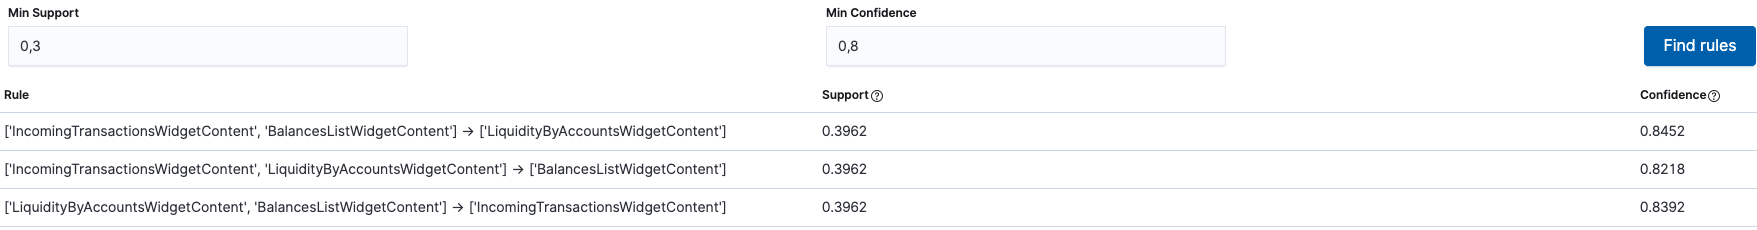
\includegraphics[width=430pt]{bilder/associationrules_result.png}
\end{center}
\caption{Ergebnis der Suche nach Assoziationsregeln}
\label{fig:associationrule-result}
\end{figure}
\\
Wie sich erkennen lässt, tritt das Itemset \textit{IncomingTransactionWidgetContent, BalancesWidgetContent} und \textit{LiquidityByAccountsWidgetContent} bzgl. des angegebenen minsupports häufig auf. Desweiteren stellen die Regeln eine Permutation dar, in der jedes Widget ein Mal als Konsequenz vorkommt. Daraus lässt sich ableiten, dass die Implementierung zum Finden der Assoziationsregeln korrekt funktioniert.\\
Aus der Analyse des Speicherverbrauchs resultieren die folgenden Plots:\\
\clearpage
\begin{figure}[htb]
\begin{center}
	\begin{subfigure}{0.47\textwidth}
		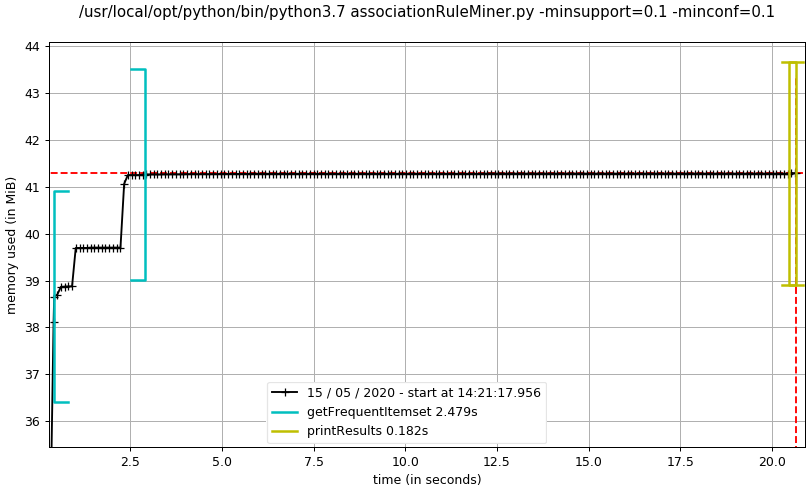
\includegraphics[width=\textwidth]{bilder/ass-conf-0101.png}
		\caption{}
		\label{subfig:0101}
	\end{subfigure}\qquad
	\begin{subfigure}{0.47\textwidth}
		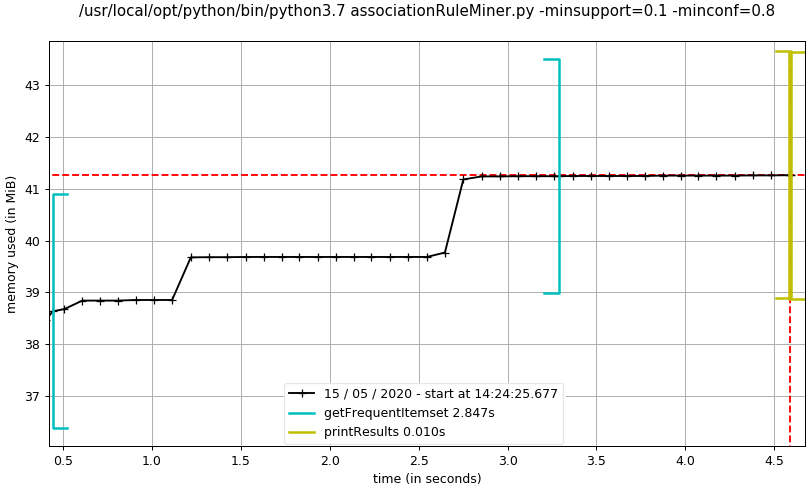
\includegraphics[width=\textwidth]{bilder/ass-conf-0108.png}
		\caption{}
		\label{subfig:0108}
	\end{subfigure}\\
	\begin{subfigure}{0.47\textwidth}
		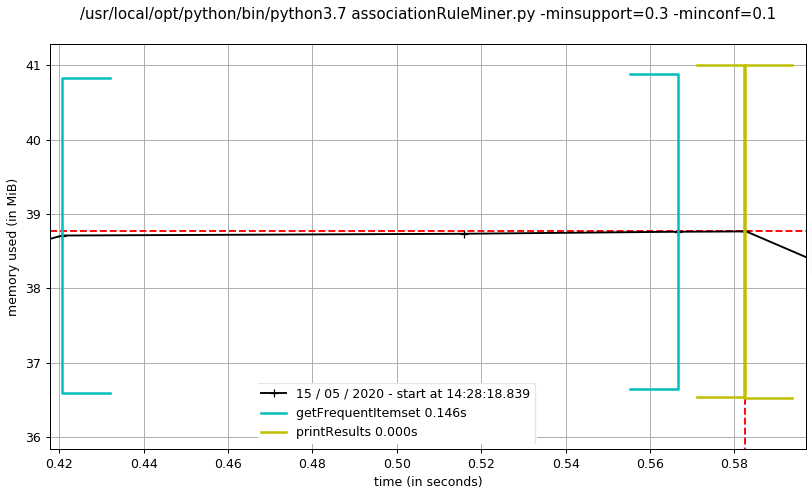
\includegraphics[width=\textwidth]{bilder/ass-conf-0301.png}
		\caption{}
		\label{subfig:0301}
	\end{subfigure}\qquad
	\begin{subfigure}{0.47\textwidth}
		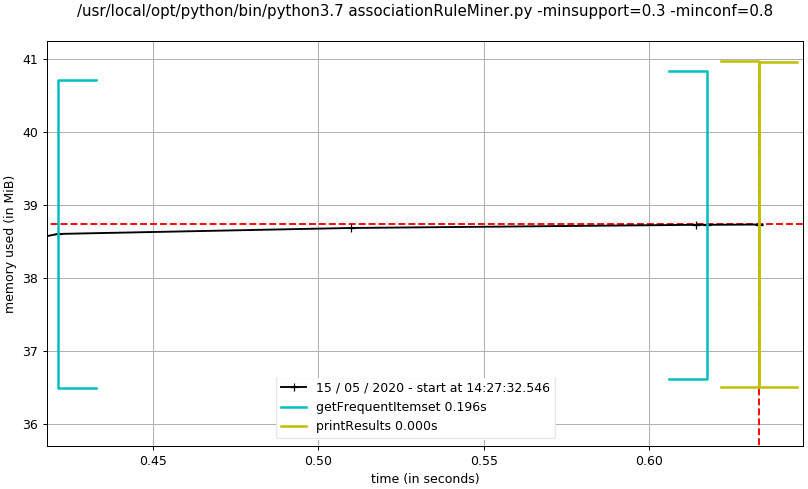
\includegraphics[width=\textwidth]{bilder/ass-conf-0308.png}
		\caption{}
		\label{subfig:0308}
	\end{subfigure}
\end{center}
\caption{Ergebnis Speicheranalyse}
\label{fig:result-mem-analysis}
\end{figure}
Die Plots zeigen den Speicherverbrauch ab dem Zeitpunkt, an dem die häufigen Itemsets bestimmt werden (blaue Klammer) bis zur Ausgabe der gefundenen Regeln (gelbe Klammer)\footnote{Für die Generierung der Assoziationsregeln wurde nicht direkt die Speichernutzung gemessen, sondern durch die Funktionen getFrequentItemsets und printResults eingegrenzt. Diese Funktionen werden unmittelbar vor bzw. nach der Generierung der Regeln aufgerufen. Der Grund für diese Vorgehensweise ist, dass \textproc{memory\_profiler} pro Funktionsaufruf eine Klammer darstellt. Da die Regeln rekursiv gefunden werden, wären zu viele Klammern in dem Plot erschienen, was die Lesbarkeit stark einschränkt.} an. Der Bereich zwischen den Klammern stellt den Speicherverbrauch während der Generierung der Regeln dar. Die Parameter für die Werte minsupport und minkonfidenz wurden so gewählt, dass sie einmal einen eher schlecht gewählten Wert bekommen (0.1) und entsprechend passendere Werte (minsupport = 0.3, minkonfidenz = 0.8). Es ist trivial, dass sich der gewählte minsupport auf die blaue Klammer auswirkt und die minkonfidenz auf die gelbe Klammer. Allerdings wirkt sich ein unpassend gewählter minsupport vergleichsweise stark auf die Speichernutzung aus. Vergleichen wir dazu einmal Abbildung \ref{subfig:0108} und Abbildung \ref{subfig:0308}. Wie sich deutlich erkennen lässt, wird bei einem niedrigen minsupport wesentlich mehr Speicher benötigt, da mehr Kandidaten für häufige Itemsets betrachtet werden müssen. Dementsprechend dauert es auch länger alle häufigen Itemsets zu bestimmen. Betrachtet man den Bereich zwischen der blauen und gelben Klammer, der die Generierung der Regeln darstellt, lässt sich festestellen, dass sich die Wahl der minkonfidenz mehr auf die benötigte Zeit auswirkt, um Regeln zu finden, als auf die Speichernutzung. Das sieht man besonders, wenn man Abbildung \ref{subfig:0101} und Abbildung \ref{subfig:0108} miteinander vergleicht: im ersten Fall müssen wesentlich mehr Funktionsaufrufe getätigt werden, erkennbar an den schwarzen, senkrechten Strichen auf der schwarzen Linie.

\subsubsection{Diskussion}
\label{ssub:Diskussion}
In diesem Abschnitt sollen die Ergebnisse aus Kapitel \ref{ssub:Resultate} kritisch diskutiert werden.\\
Wenden wir uns dazu zunächst den Visualisierungen zu. Anscheinend ist es für die Visualisierung nicht zwingend notwendig, die Daten zu transformieren. Das folgt aus der Tatsache, dass es Möglich war, das selbe Diegramm aus zwei verschiedenen Indices zu erstellen.\\
Dennoch hat die Transformierung den Vorteil, Daten in einem Format zu zeigen, welches sich für weitere Analyseverfahren in Bereich \textit{Knowledge Discovery in Databases} (KDD) eignet. Denkbar wäre hier die Anwendung der Nächste-Nachbarn-Klassifikation \citep{EsSa00} auf die Arrays, welche die Widgetnutzung pro Session speichern.\\
Im Bezug auf die Suche nach den Assoziationsregeln war es ebenfalls von Vorteil, die Daten transformiert zu betrachten. Durch die transformation hat ein besseres Verständnis über Daten erhalten.
%Mit Hilfe der Pie Diagramme wird gezeigt, dass die Daten richtig transformiert wurden und die Lines Visualisierung den Verlauf der Nutzung der Widgets ebenfalls korrekt darstellt. Daraus lässt sich schließen, dass für die Visualisierung an sich nicht zwingend notwendig ist, die Daten zu transformieren. Dennoch hat die Transformierung den Vorteil, dass die Daten in einem Format sind, das sich für weitere Analyseverfahren in Bereich \textit{Knowledge Discovery in Databases} (KDD) eignet. Denkbar wäre z.B. dass man auf die Arrays, die die Widgetnutzung pro Session speichern, die \textit{Nächste-Nachbarn-Klassifikation} \citep{EsSa00} anwendet.\\
\newline
Bevor die Ergebnisse der Assoziationsregelnanalyse diskutiert werden, ist es wichtig zu klären, welche Information eine Assoziationsregel genau liefert. Nach \citet{BeKe19} kann man den minsupport als relative Häufigkeit und die minkonfidenz als die Wahrscheinlichkeit einer Regel betrachten. Vergleichen wir dazu die erste Regel aus Abbildung \ref{fig:associationrule-result}. Diese Regel sagt aus, dass in 39.62\% aller Sessions die Widgets \textit{IncomingTransactionWidgetContent, BalancesWidgetContent} und \textit{LiquidityByAccountsWidgetContent} zusammen vorkommen. Mit einer Wahrscheinlichkeit von 84.52\% wird \textit{LiquidityByAccountsWidgetContent} angeklickt, wenn die anderen beiden Widgets benutzt wurden. Die Assoziationsregel suggeriert eine temporale Beziehung zwischen Antezedenz und Konsequenz der Regel. Tatsächlich berücksichtigt der in dieser Arbeit verwendete Algorithmus keine zeitlichen Aspekte, sodass dieser Rückschluss falsch sein kann \citep{Be03}.\\
Nichtsdestotrotz kann man bei realen Kundendaten vermuten, dass auch eine zeitliche Beziehung zwischen den Widgets besteht. Wird bspw. die Regel 
\begin{equation*}
\textit{Open Payments} \rightarrow \textit{LiquidityByAccountsWidgetContent} 
\end{equation*}
gefunden, die den minsupport und die minkonfidenz erfüllt, ist es naheliegend, dass \textit{Open Payments} zuerst benutzt wurde. Diese Interpretation basiert aber ausschließlich auf der Vermutung des Benutzers.\\
Aus dieser Feststellung folgt eine weitere Eigenschaft der Assoziationsregeln, die erwähnt werden muss. Da zeitliche Abfolgen nicht berücksichtigt werden, kann es auch durchaus sein, dass ein Workflow \glqq unterbrochen\grqq{} wird. Das bedeutet, dass zwischen der Antezedenz und Konsequenz einer Regel auch weitere Widgets benutzt worden sein können. Diese Tatsache wirkt zunächst wie eine Einschränkung für die Verwendbarkeit bzw. Aussagekraft der Assoziationsregeln. Man kann dies aber auch als Vorteil betrachten, da der Algorithmus Workflows trotz Unterbrechungen findet. So könnte eine Unterbrechung z.B. aus Versehen zustande kommen, indem sich ein User \glqq verklickt\grqq{} hat.\\
Mit Blick auf die Aufgabenstellung aus Kapitel \ref{sub:Problemstellung} lässt sich also zusammenfassen, dass die Suche nach Assoziationsregeln Workflows erkennen kann, mit der Voraussetzung, dass zeitliche Aspekte nicht berücksichtigt werden.
\clearpage
